\documentclass{article}

\usepackage{graphicx}
\usepackage{tabularx}
\usepackage{setspace}
\usepackage{amssymb}
\usepackage{amsmath}
\usepackage[b5paper, portrait, top=2.5cm, bottom=2.5cm, left=2.5cm, right=2.5cm]{geometry}

\begin{document}
	{\setstretch{1.0}
		\large
		\thispagestyle{empty}
		\begin{flushleft}
			
\includegraphics[width=90px]{lambang-its-color-std.png}\\
			{\fontfamily{cmss}\selectfont
				\vspace{4cm}
				GROUP HOMEWORK\\
				INTRODUCTORY FINANCIAL MATHEMATICS CLASS - SM141432\\
				\vspace{0.2cm}
				\textbf{2nd HOMEWORK}\vspace{0.4cm}
				
				\begin{minipage}{10cm}
					\flushleft
					NOVITA PUSPITASARI\\NRP 0611 1540000 011\\ \vspace{0.15cm}
					VENANSIUS RYAN TJAHJONO\\NRP 0611 1540000 043\\ \vspace{0.15cm}
					YUSRIL IZZA FRIZNAINI\\NRP 0611 1540000 048\\ \vspace{0.15cm}
					WINDA FIRDIANA\\NRP 0611 1540000 051\\ \vspace{0.15cm}
				\end{minipage}
				\\
				\vspace{1cm}
				Lecturer: \\
				Endah Rokhmati Merdika Putri, S.Si, M.T, Ph.D\\
				\vspace{1cm}
				\textbf{DEPARTMENT OF MATHEMATICS}\\
				Faculty of Mathematics, Computing, and Data Science\\
				Institut Teknologi Sepuluh Nopember\\
				Surabaya 2018\\
			}
		\end{flushleft}
	}
	\pagebreak
	\begin{center}
		\textbf{QUESTIONS}
	\end{center}
	\begin{enumerate}
		\item \textbf{Example 1.3} (\textit{Compound interest calculation})\\ 
		Smith deposits 1000 into an account on January 1, 2005. The account credits interest at an effective annual rate of 5\% every December 31. Smith withdraws 200 on January 1, 2007, deposits 100 on January 1, 2008, and withdraws 250 on January 1, 2010. What is the balance in the account just after interest is credited on December 31, 2011?
		
		\item \textbf{Exercise 1.1.3}\\ 
		Bob puts 10,000 into a bank account that has monthly compounding with interest credited at the end of each month. The monthly interest rate is 1\% for the first 3 months of the account and after that the monthly interest rate is .75\%. Find the balance in Bob's account at the end of 12 months just after interest has been credited. Find the average compound monthly interest rate on Bob's account for the 12 month period.
		
		\item \textbf{Exercise 1.1.4S}\\
		Carl puts 10,000 into a bank account that pays an effective annual interest rate of 4\% for ten years, with interest credited at the end of each year. If a withdrawal is made during the first five and one-half years, a penalty of 5\% of the withdrawal is made. Carl withdraws \textit{K} at the end of each of years 4,5,6 and 7. The balance in the account at the end of year 10 is 10,000. Calculate $K$.
		
		\item \textbf{Exercise 1.1.5}
		\begin{enumerate}
			\item[(a)] Unit values in a mutual fund have experienced annual growth rates of 10\%, 16\%, -7\%, 4\%, and 32\% in the past five years. The fund manager suggest the fund can advertise an average annual growth of 11\% over the past five years. What is the actual average annual compound growth rate over the past five years?
			\item[(b)] A mutual fund advertises that average annual compound rate of returns for various periods ending December 31, 2005 are as follows:\\
			10 years - 13\%; 5 years - 17\%; 2 years - 15\%; 1 year - 22\%.\\
			Find the 5-year average annual compound rates of return for the period January 1, 1996 to December 31, 2000, and find the annual rate of return for calender year 2004.
		\end{enumerate}
	\end{enumerate}
	
	\pagebreak
	\begin{center}
		\textbf{SOLUTIONS}
	\end{center}
	\begin{enumerate}
		\item \textbf{Example 1.3} (\textit{Compound interest calculation})\\
		Based on the question above, we know that effective annual rate is 5\% every 31$^{st}$ December and Smith deposits \$1000 at first. To make calculation easier, lets take a look for the table below. 
		\begin{center}
			\begin{tabular}{|c|c|c|c|c|}
				\hline
				\textbf{Date}&\textbf{Debit}(\$)&\textbf{Credit}(\$)&\textbf{Calculation}&\textbf{Balance}(\$)\\\hline
				01/01/05&0&1000&$0+1000$&1000\\\hline
				31/12/05&0&50&$1000+50$&1050\\\hline
				31/12/06&0&52.5&$1050+52.5$&1102.50\\\hline
				01/01/07&200&0&$1102.50-200$&902.50\\\hline
				31/12/07&0&45.13&$902.50+45.13$&947.63\\\hline
				01/01/08&0&100&$947.63+100$&1047.63\\\hline
				31/12/08&0&52.38&$1047.63+52.38$&1100.01\\\hline
				31/12/09&0&55&$1100.01+55$&1155.01\\\hline
				01/01/10&250&0&$1155.01-205$&905.01\\\hline
				31/12/10&0&45.25&$905.01+45.25$&950.26\\\hline
				31/12/11&0&47.51&$950.26+47.51$&997.77\\\hline
			\end{tabular}
		\end{center}
		Based on our calculation above, Smith's balance in his account just after interest is credited on December 31, 2011 is \textbf{\$997.77}.
		\item \textbf{Exercise 1.1.3}\\
		Note that, Bob's Bank has different regulation in different month. It is said that:
		\begin{enumerate}
			\item[a.] The monthly interest rate is 1\% for the first three months.
			\item[b.] The monthly interest rate is .75\% after the first three months.
		\end{enumerate} 
		Total Bob's balance in the end of 12 months just after interest has been credited is:
		$$\$10000\times(1.01)^3\times(1.0075)^9=\textbf{\$11019.696}$$
		Average compound monthly interest rate for 12 months period is $j$ where: 
		\begin{center}
			\begin{tabular}{rcl}
				$10000(1+j)^{12}$&=&11019.696\\
				$(1+j)^{12}$&=&1.1019696\\
				$1+j$&=&$(1.1019696)^{1/12}$\\
				$1+j$&=&1.0081244\\
				$j$&=&0.0081244 $\approx0.812\%$\\
			\end{tabular}
		\end{center}
		
		In conclusion, the average compound monthly interest rate is \textbf{0.812\%}
		
		\pagebreak
		\item \textbf{Exercise 1.1.4S}\\
		Let's simplified the problem by listing the events as follows.
		\begin{enumerate}
			\item[i.] Carl put \$10000 into a bank with interest rate 4\% for ten years, credited at the end of each year.
			\item[ii.] If withdrawal is made during first $5\frac{1}{2}$ years, Carl will have penalty 5\% of the withdrawal is made.
			\item[iii.] Carl withdraws $K$ at the end of each years 4, 5, 6, and 7. It means that he will have penalty 5\% for withdrawal at the end of year 4 and 5.
			\item The balance inquiry at the end of year 10 is \$10000.
		\end{enumerate}
		To find Carl's withdrawal $K$, we have to list what happened during 10 years as follows. (\textit{Assume that, Carl withdraws money after the interest has been credited})
		\begin{enumerate}
			\item \textbf{Years 1-4}. At the end of year 4, Carl's balance is $10000(1.04)^4$. In the end of year 4, Carl withdraws $K$ (Carls got a penalty 5\%), it means that the Carl's balance is $10000(1.04)^4-K(1.05)$.
			\item \textbf{Year 5}. At the end of year 5, Carl's balance is $(10000(1.04)^4-K(1.05))(1.04)$. After that, Carl withdraws $K$ again (Carls got a penalty 5\%), so the Carl's balance is $(10000(1.04)^4-K(1.05))(1.04)-K(1.05)$.
			\item \textbf{Year 6}. At the end of year 6, interest rate credited 4\%, so Carl's balance is $((10000(1.04)^4-K(1.05))(1.04)-K(1.05))(1.04)$. Then, Carl withdraws $K$ (he wont get penalty because he withdraws at year 6), so the Carl's balance is $((10000(1.04)^4-K(1.05))(1.04)-K(1.05))(1.04)-K$.
			\item \textbf{Year 7}. Same as year 6, after interest rate credited, Carl withdraws $K$, so the Carl's balance is $(((10000(1.04)^4-K(1.05))(1.04)-K(1.05))(1.04)-K)(1.04)-K$.
			\item \textbf{Year 8-10}. Carl doesn't withdraw any. So, his balance at the end of year 10 after interest rate has been credited is $((((10000(1.04)^4-K(1.05))(1.04)-K(1.05))(1.04)-K)(1.04)-K)(1.04)^3$. This amount equals to \$10000.
		\end{enumerate}
		
		By using Microsoft Mathematics software, we solve the equation and we have $K=\textbf{\$979.93}$\vspace{-0.4cm}
		\begin{center}
			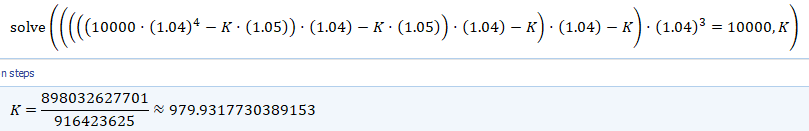
\includegraphics[width=350px]{num3.png}
		\end{center}
	
		\pagebreak
		\item \textbf{Exercise 1.1.5}\\
		\begin{enumerate}
			\item[(a)] Over five years, the unit value has grown 10\%, 16\%, $-$7\%, 4\%, and 32\%. Because the growth is corresponding with geometric series, we think it is more suitable if we use geometric means to calculate average growth.\\
			
			Firstly, we count the total growth for past five years as follows: $$(1+.10)(1+.16)(1+(-.07))(1+.04)(1+.32)=1.6291$$
			Secondly, by applying geometric means we will have:
			$$1.6291^{1/5}=1.1025$$
			It means that the average growth for past five years is \textbf{10.25\%}.
			
			\vspace{0.3cm}
			\item[(b)] First of all, let's assume the money in this case is 1. Based on the case above, we know that annual compound rates of return for various periods ending Dec 31$^{st}$, 2005 is as follows.\vspace{0.1cm}\\
			\begin{tabular}{lcc}
				\textbf{10 years} (1996$-$2005)&:& 13\%\\
				\textbf{5 years} (2001$-$2005)&:& 17\%\\
				\textbf{2 years} (2004$-$2005)&:& 15\%\\
				\textbf{1 years} (return in 2005)&:& 22\%
			\end{tabular}
			\vspace{0.5cm}\\
			\textbf{Case 1: 5 year average annual return starting Jan 1, 1996 until Dec 31$^{st}$, 2000.} It is starting at Jan 1, 1996 and ending at Dec 31$^{st}$, 2005, it means we have interval 10 years. So, the money at the end of year 10 is $(1.13)^{10}$. Then, the money at the end of year 5 (Dec 31$^{st}$, 2000) is $(1.17)^{5}$. Assume the average annual rate of return is $p$ where: $$(1.17)^5(1+p)^5=(1.13^{10})$$ By using Microsoft Mathematics, we have $p\approx0.0913675=\textbf{9.14\%}$.\\
			\begin{center}
				\includegraphics[width=200px]{num4b.png}
			\end{center}
			\vspace{0.5cm}
			\textbf{Case 2: Annual rate of return for calendar 2004.} Based on the information above, the money at the end of year 2005 is $(1.15)^2$ and at the end of year 2004 is $1.22$. The value of average annual rate of return is $q$ where: $$(1.22)(1+q)=(1.15)^2$$ By using simple mathematics, $q=\frac{(1.15)^2}{1.22}-1=0.084016393$.\\ In conclusion we have $q\approx$ \textbf{8.401\%}.
		\end{enumerate}
	\end{enumerate}
\end{document}